% =============================================================================
%  The HACA Broadcast Transcription System
%  Architecture, Pipelines, and Tooling
%
%  Self-contained Overleaf document. Compile with pdfLaTeX (run twice for the
%  table of contents and cross-references). No external images required -- all
%  diagrams are drawn with TikZ.
% =============================================================================
\documentclass[11pt,a4paper]{report}

% ---- Page geometry & fonts -------------------------------------------------
\usepackage[utf8]{inputenc}
\usepackage[T1]{fontenc}
\usepackage{lmodern}
\usepackage[a4paper,margin=2.5cm]{geometry}
\usepackage{microtype}

% ---- Colour, tables, lists -------------------------------------------------
\usepackage{xcolor}
\usepackage{booktabs}
\usepackage{tabularx}
\usepackage{array}
\usepackage{enumitem}
\usepackage{longtable}

% ---- Headers / footers -----------------------------------------------------
\usepackage{fancyhdr}
\pagestyle{fancy}
\fancyhf{}
\fancyhead[L]{\nouppercase{\leftmark}}
\fancyhead[R]{\thepage}
\renewcommand{\headrulewidth}{0.4pt}

% ---- Diagrams --------------------------------------------------------------
\usepackage{tikz}
\usetikzlibrary{arrows.meta,positioning,shapes.geometric,fit,backgrounds,calc}

% ---- Hyperlinks (load late) ------------------------------------------------
\usepackage[hidelinks,colorlinks=true,linkcolor=blue!55!black,
            urlcolor=blue!55!black,citecolor=blue!55!black]{hyperref}

% ---- Code listings ---------------------------------------------------------
\usepackage{listings}

\definecolor{codebg}{rgb}{0.97,0.97,0.97}
\definecolor{codeframe}{rgb}{0.85,0.85,0.85}
\definecolor{kw}{rgb}{0.13,0.29,0.53}
\definecolor{str}{rgb}{0.16,0.50,0.16}
\definecolor{cmt}{rgb}{0.50,0.50,0.50}
\definecolor{num}{rgb}{0.60,0.30,0.00}

\lstdefinestyle{py}{
  language=Python,
  backgroundcolor=\color{codebg},
  basicstyle=\ttfamily\footnotesize,
  keywordstyle=\color{kw}\bfseries,
  stringstyle=\color{str},
  commentstyle=\color{cmt}\itshape,
  numberstyle=\tiny\color{cmt},
  identifierstyle=\color{black},
  numbers=left,
  numbersep=7pt,
  frame=single,
  rulecolor=\color{codeframe},
  breaklines=true,
  showstringspaces=false,
  tabsize=4,
  captionpos=b,
  columns=fullflexible,
}

\lstdefinestyle{sh}{
  backgroundcolor=\color{codebg},
  basicstyle=\ttfamily\footnotesize,
  commentstyle=\color{cmt}\itshape,
  frame=single,
  rulecolor=\color{codeframe},
  breaklines=true,
  showstringspaces=false,
  columns=fullflexible,
}

\lstset{style=py}

% Inline code shortcut.
\newcommand{\code}[1]{\texttt{\small #1}}

% ---- Title metadata --------------------------------------------------------
\title{\textbf{The HACA Broadcast Transcription System}\\[0.4em]
       \large Architecture, Pipelines, and Tooling\\[0.3em]
       \normalsize A complete technical reference for the \texttt{transcription/} repository}
\author{HACA --- Broadcast Transcription}
\date{\today}

% =============================================================================
\begin{document}

\maketitle

\begin{abstract}
\noindent
This document is a complete technical reference for the \texttt{transcription}
repository: an open-source system that turns radio and television broadcasts in
\textbf{Moroccan Darija}, \textbf{Modern Standard Arabic}, and \textbf{French}
--- including recordings that \emph{code-switch} between all three within a
single clip --- into standard \texttt{.srt} subtitle files.

The system is built on \href{https://github.com/SYSTRAN/faster-whisper}{faster-whisper}
(OpenAI's Whisper served through the CTranslate2 inference engine), augmented
with \textbf{per-chunk language detection} so that mixed-language audio is
transcribed natively rather than being forced into one language, and with an
optional \textbf{Darija LoRA adapter} that markedly improves Moroccan-Arabic
accuracy. A second, richer pipeline based on
\href{https://github.com/m-bain/whisperX}{WhisperX} adds word-level alignment and
speaker diarization.

Around these two pipelines sits a reusable \texttt{core} package and a batch
command-line tool that selects files from a structured media archive, transcribes
them, and writes a mirrored tree of subtitles. We document every module,
function, algorithm, configuration option, data format, test, and deployment path
(including GPU Docker images), so that a new contributor can understand the entire
codebase from this single document.
\end{abstract}

\tableofcontents

% #############################################################################
\chapter{Introduction}
% #############################################################################

\section{What this repository does}

The \texttt{transcription} repository is a \emph{standalone tool}. Given a media
file (audio or video) of a broadcast, it produces a standard SubRip subtitle file
(\texttt{.srt}) containing time-stamped text cues. Its defining characteristic is
that it handles \textbf{code-switching}: a single Moroccan news bulletin or talk
show routinely mixes Darija, Modern Standard Arabic (MSA), and French --- often
within the same sentence. Conventional usage of Whisper forces a single language
for an entire file, which mistranscribes the other languages. This project instead
detects the language of each short \emph{chunk} of audio independently, so each
segment is transcribed in the language actually being spoken.

\section{The Darija problem}

Whisper's weakest area among the languages of interest is Darija (Moroccan
Arabic), which it represents internally as generic Arabic (\code{ar}) and often
transcribes poorly. The repository addresses this in two complementary ways:

\begin{itemize}[leftmargin=1.4em]
  \item \textbf{Constrained language detection.} Auto-detection is restricted to
        an allow-list (default \code{ar,fr,en}); anything off-list falls back to
        \code{ar}. This keeps noisy Moroccan speech from drifting to spurious
        languages.
  \item \textbf{A Darija LoRA adapter.} The
        \href{https://huggingface.co/anaszil/whisper-large-v3-turbo-darija}{\code{anaszil/whisper-large-v3-turbo-darija}}
        adapter (a LoRA on \code{large-v3-turbo}) is benchmarked as both faster and
        more accurate than full \code{large-v3} fine-tunes on real broadcast audio.
        When enabled, only the chunks detected as Arabic are routed through it; the
        base model still handles French and English.
\end{itemize}

\section{Two pipelines}

The repository ships two transcription pipelines that share the same front-half
philosophy (decode, segment, per-chunk language detection) but differ in their
back-half capabilities:

\begin{description}[leftmargin=2em,style=nextline]
  \item[\texttt{src/transcribe.py} (faster-whisper)] The default, lighter
        pipeline. Decodes, runs Voice-Activity-Detection (VAD) chunking, detects
        language per chunk, transcribes, and writes \texttt{.srt}. No speaker
        labels.
  \item[\texttt{src/transcribe\_whisperx.py} (WhisperX)] A heavier pipeline that
        additionally performs \emph{word-level alignment} (wav2vec2, per language)
        and \emph{speaker diarization} (pyannote), prefixing each cue with a
        speaker tag such as \code{[SPEAKER\_00]}.
\end{description}

\section{Output is the contract}

The project deliberately produces nothing but standard \texttt{.srt}. That single
choice keeps it decoupled from every downstream consumer: the separate HACA
sentiment/tonality benchmark, a video player, or any subtitle tool can read the
output without sharing a line of code with this repository. The two projects are
interoperable \emph{through the file format alone}.

\section{Audience and scope}

This document covers the \texttt{transcription} repository in full. A companion
web application (an Angular front-end with a FastAPI backend, the
``Transcription UI'') is \emph{planned} and reuses the same \texttt{core} package;
it is referenced where relevant but not documented in depth here. The broader HACA
benchmark is likewise mentioned only as a downstream consumer.

% #############################################################################
\chapter{Repository Layout}
% #############################################################################

The repository is organised into the existing single-file pipelines
(\texttt{src/}), a shared \texttt{core/} package, a batch CLI (\texttt{cli.py}),
documentation, notebooks for GPU runners, tests, and container files.

\begin{lstlisting}[style=sh,numbers=none,caption={Annotated repository tree.}]
transcription/
|-- cli.py                     # Batch CLI over a medias/ tree (filters -> mirrored out/srt/)
|-- core/                      # Shared logic, imported by the CLI and the (planned) web UI
|   |-- __init__.py            #   re-exports the config symbols
|   |-- config.py              #   TranscribeConfig dataclass + defaults + validation
|   |-- selection.py           #   range parsing, medias scan, expand_selections()
|   |-- runner.py              #   load models once, run_file(), mirrored SRT, error capture
|   `-- summary.py             #   FileResult, RunSummary, structured log formatting
|-- src/                       # The transcription pipelines (the heavy lifting)
|   |-- transcribe.py          #   faster-whisper pipeline + its own CLI
|   |-- transcribe_whisperx.py #   WhisperX pipeline (alignment + diarization) + its own CLI
|   `-- srt_writer.py          #   standard .srt writer (shared by everything)
|-- tests/                     # pytest suite (no GPU/model needed)
|   |-- test_srt_writer.py
|   |-- test_config.py
|   |-- test_selection.py
|   |-- test_runner.py
|   `-- test_cli.py
|-- docs/                      # Documentation
|   |-- PIPELINE.md            #   comprehensive pipeline reference
|   |-- TRANSCRIPTION.md       #   design notes (why faster-whisper, the Darija reality)
|   |-- WHISPERX_GUIDE.md      #   WhisperX deep-dive
|   |-- CLI_ARCHITECTURE.md    #   batch CLI architecture + Docker guide
|   `-- transcription_report.tex  # (this document)
|-- notebooks/                 # Kaggle/Colab GPU runners and model comparisons
|-- samples/                   # A few example broadcast clips for smoke tests
|-- requirements.txt           # faster-whisper + transformers + peft (LoRA)
|-- requirements_whisperx.txt  # whisperx + pyannote (only for the WhisperX pipeline)
|-- Dockerfile.gpu             # GPU image for the batch CLI
|-- docker-compose.yml         # convenience wrapper for repeated GPU runs
`-- .dockerignore
\end{lstlisting}

\noindent
The remaining chapters work bottom-up and then top-down: first the concepts shared
by both pipelines (Chapter~\ref{ch:fundamentals}), then each pipeline in detail
(Chapters~\ref{ch:fw}--\ref{ch:srt}), then the shared \texttt{core} package
(Chapter~\ref{ch:core}) and the CLI that ties it together
(Chapter~\ref{ch:cli}), and finally testing, deployment, and reference material.

% #############################################################################
\chapter{High-Level Architecture}
\label{ch:arch}
% #############################################################################

\section{The layered design}

The system is organised into three layers. At the bottom are the
\emph{pipelines} (\texttt{src/}) that actually perform speech recognition. In the
middle is a reusable \emph{core} package that knows how to configure a run, decide
which files to process, drive a pipeline over many files, and record results. At
the top are \emph{front-ends} that a human (or another service) interacts with:
the batch CLI today, and a planned web UI. The key architectural rule is that both
front-ends depend only on \texttt{core}, and \texttt{core} wraps \texttt{src} ---
so the CLI and the web UI can never diverge in behaviour.

\begin{figure}[ht]
\centering
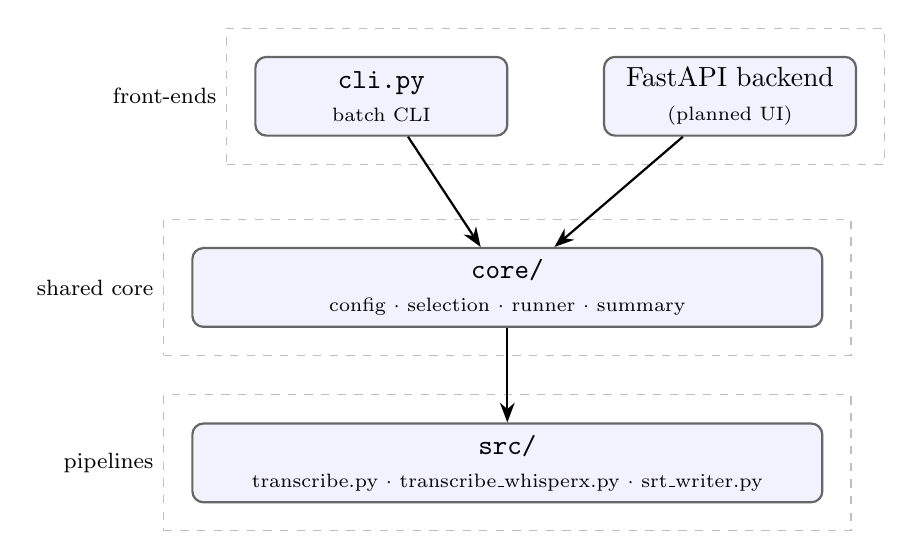
\begin{tikzpicture}[
   node distance=0.9cm and 1.2cm,
   box/.style={rectangle, rounded corners, draw=black!60, thick,
               align=center, minimum height=1cm, minimum width=3.2cm,
               fill=blue!5},
   layer/.style={rectangle, draw=black!25, dashed, inner sep=0.35cm},
   arr/.style={-{Stealth[length=2.5mm]}, thick}
]
% Front-ends
\node[box] (cli) {\texttt{cli.py}\\\scriptsize batch CLI};
\node[box, right=of cli] (ui) {FastAPI backend\\\scriptsize (planned UI)};
% Core
\node[box, below=1.4cm of cli, minimum width=8.0cm, xshift=1.6cm] (core)
     {\texttt{core/}\\\scriptsize config $\cdot$ selection $\cdot$ runner $\cdot$ summary};
% Pipelines
\node[box, below=1.2cm of core, minimum width=8.0cm] (src)
     {\texttt{src/}\\\scriptsize transcribe.py $\cdot$ transcribe\_whisperx.py $\cdot$ srt\_writer.py};

\draw[arr] (cli) -- (core);
\draw[arr] (ui) -- (core);
\draw[arr] (core) -- (src);

\begin{scope}[on background layer]
  \node[layer, fit=(cli)(ui), label=left:{\footnotesize front-ends}] {};
  \node[layer, fit=(core), label=left:{\footnotesize shared core}] {};
  \node[layer, fit=(src), label=left:{\footnotesize pipelines}] {};
\end{scope}
\end{tikzpicture}
\caption{The three-layer architecture. Front-ends depend on \texttt{core};
\texttt{core} wraps the \texttt{src} pipelines.}
\label{fig:layers}
\end{figure}

\section{Two design principles that make it robust}

\paragraph{Lazy heavy imports.} The faster-whisper / WhisperX stack is imported
only \emph{inside} the functions that actually transcribe, never at module import
time. As a result, importing \texttt{core} --- and running selection, configuration,
and \code{--dry-run} logic --- works with nothing but the Python standard library
installed. This keeps start-up fast and, crucially, lets the entire test suite run
without a GPU or a multi-gigabyte model download.

\paragraph{Injection seams.} The function that transcribes one file,
\code{core.runner.run\_file}, accepts optional \code{transcribe\_fn} and
\code{write\_fn} parameters. Production code passes neither and the real models
run; tests pass lightweight fakes. Every path-handling and error-handling branch
is therefore testable in isolation.

\section{End-to-end data flow}

Figure~\ref{fig:flow} traces a batch run from the command line to the subtitle
files on disk.

\begin{figure}[ht]
\centering
\begin{tikzpicture}[
   node distance=0.55cm,
   step/.style={rectangle, rounded corners, draw=black!60, thick,
                align=left, text width=11.5cm, fill=gray!4,
                inner sep=0.25cm},
   arr/.style={-{Stealth[length=2.2mm]}, thick}
]
\node[step] (s1) {\textbf{1. Parse arguments} --- \code{cli.build\_parser().parse\_args()}};
\node[step, below=of s1] (s2) {\textbf{2. Parse filters} --- \code{parse\_channels()}, \code{parse\_ranges()} \hfill\textit{core.selection}};
\node[step, below=of s2] (s3) {\textbf{3. Build + validate config} --- \code{config\_from\_args()} $\to$ \code{TranscribeConfig.validate()} \hfill\textit{core.config}};
\node[step, below=of s3] (s4) {\textbf{4. Expand selection} --- \code{expand\_selections()} produces the file list \hfill\textit{core.selection}\\[2pt]\hspace{1em}$\hookrightarrow$ if \code{--dry-run}: print the list and stop};
\node[step, below=of s4] (s5) {\textbf{5. Load models once} --- \code{runner.load\_models(config)} \hfill\textit{core.runner $\to$ src}};
\node[step, below=of s5] (s6) {\textbf{6. For each file} --- \code{runner.run\_file()}: skip-if-exists, transcribe, write mirrored \texttt{.srt}, capture failures; append a log line \hfill\textit{core.runner / summary}};
\node[step, below=of s6] (s7) {\textbf{7. Finish} --- write \code{[JOB END]}, print one-line summary, return exit code};

\draw[arr] (s1)--(s2); \draw[arr] (s2)--(s3); \draw[arr] (s3)--(s4);
\draw[arr] (s4)--(s5); \draw[arr] (s5)--(s6); \draw[arr] (s6)--(s7);
\end{tikzpicture}
\caption{End-to-end flow of a batch run. Per-file failures never abort the batch;
they are recorded and the run continues.}
\label{fig:flow}
\end{figure}

% #############################################################################
\chapter{Pipeline Fundamentals}
\label{ch:fundamentals}
% #############################################################################

Both pipelines share a seven-stage shape. Understanding these stages once makes
both \texttt{transcribe.py} and \texttt{transcribe\_whisperx.py} easy to read.

\begin{enumerate}[leftmargin=1.6em]
  \item \textbf{Decode} the media file to a 16\,kHz mono \code{float32} waveform.
  \item \textbf{VAD segmentation}: find regions of speech with Voice Activity
        Detection.
  \item \textbf{Chunking}: group speech regions into chunks of at most $\sim$25
        seconds, breaking only at silence.
  \item \textbf{Per-chunk language detection}, constrained to an allow-list.
  \item \textbf{Transcribe} each chunk in its detected language.
  \item \textbf{Collect} segments and shift their timestamps to absolute time.
  \item \textbf{Write} a standard \texttt{.srt}.
\end{enumerate}

\section{Stage 1 --- Decoding to 16\,kHz mono}

Whisper models expect 16\,kHz mono audio. Decoding is delegated to the
pipeline's backend: faster-whisper uses \href{https://pyav.org/}{PyAV} (the FFmpeg
libraries packaged as a Python wheel), while WhisperX shells out to the
\code{ffmpeg} binary. Both extract the audio track from video containers, which is
why the same code transcribes \code{.mp4} as readily as \code{.mp3}. The constant
\code{SAMPLE\_RATE = 16000} is used throughout to convert between sample indices
and seconds.

\section{Stages 2--3 --- VAD and silence-aware chunking}

Whisper degrades on very long inputs and benefits from being fed coherent spans of
speech. The pipeline therefore uses the \textbf{Silero VAD} (bundled with
faster-whisper) to find speech regions, then groups those regions into chunks.

The subtlety, explained in detail in Chapter~\ref{ch:fw}, is that Silero's default
maximum speech duration is effectively infinite, so a continuous broadcast comes
back as a single enormous region. The pipeline caps the region length at the chunk
budget and additionally hard-splits any region that still exceeds the budget, so
no audio is ever silently dropped. The grouping then extends a chunk only while it
stays within the budget, and otherwise starts a new chunk --- ensuring breaks fall
at natural pauses.

\section{Stage 4 --- Per-chunk language detection (the heart of the system)}

For each chunk, the model's language detector is run and the result is constrained
to an allow-list (default \code{ar,fr,en}); off-list detections fall back to
\code{ar}. This per-chunk decision is what enables faithful transcription of
code-switched broadcasts: a French sound-bite inside an Arabic bulletin is
detected as \code{fr} and transcribed as French, while the surrounding Darija is
transcribed as Arabic. If the user forces a language with \code{--lang}, detection
is skipped and that language is used for every chunk.

\section{Stage 5 --- Transcription (and optional Darija routing)}

Each chunk is transcribed in its chunk language. When the Darija LoRA is enabled
and the chunk language is \code{ar}, the chunk is instead routed through the LoRA
adapter (Chapter~\ref{ch:lora}); all other chunks use the base model. This routing
is per chunk and entirely automatic.

\section{Stages 6--7 --- Absolute timing and SRT output}

Each chunk carries a start offset (in seconds) into the original recording.
Segment timestamps returned by the model are relative to the chunk, so the offset
is added back to recover absolute time. The collected segments are then handed to
the SRT writer (Chapter~\ref{ch:srt}), which formats them as SubRip cues.

% #############################################################################
\chapter{The faster-whisper Pipeline (\texttt{src/transcribe.py})}
\label{ch:fw}
% #############################################################################

This is the default pipeline. It is a single file exposing both importable
functions (reused by \texttt{core.runner}) and its own command-line interface.
The heavy dependency, \code{faster\_whisper}, is imported lazily so that
\code{--help} and the SRT-writer tests work without it installed.

\section{Module-level constants}

\begin{lstlisting}[caption={Constants in \texttt{transcribe.py}.}]
MEDIA_EXTS = {
    ".mp3", ".wav", ".m4a", ".flac", ".ogg", ".opus", ".aac", ".wma",
    ".mp4", ".mkv", ".mka", ".mov", ".webm", ".avi", ".ts", ".m4v",
}
SAMPLE_RATE = 16000
DEFAULT_ALLOWED = ("ar", "fr", "en")
\end{lstlisting}

\code{MEDIA\_EXTS} is the set of audio and video extensions recognised when a
directory is batch-processed (and mirrored by the CLI's \code{core.selection},
see Chapter~\ref{ch:core}). \code{SAMPLE\_RATE} is the Whisper-required 16\,kHz.
\code{DEFAULT\_ALLOWED} is the language allow-list for auto-detection.

\section{Device and model loading}

\begin{lstlisting}[caption={Device probe and model loader.}]
def _auto_device() -> str:
    """Return 'cuda' if a GPU is visible, else 'cpu'."""
    try:
        import torch
        if torch.cuda.is_available():
            return "cuda"
    except Exception:
        pass
    try:
        import ctranslate2
        if ctranslate2.get_cuda_device_count() > 0:
            return "cuda"
    except Exception:
        pass
    return "cpu"

def load_model(model_size="large-v3", device=None, compute_type=None):
    from faster_whisper import WhisperModel
    if device in (None, "auto"):
        device = _auto_device()
    if compute_type is None:
        compute_type = "float16" if device == "cuda" else "int8"
    return WhisperModel(model_size, device=device, compute_type=compute_type)
\end{lstlisting}

\code{\_auto\_device} probes for a GPU twice: first via \code{torch} (if present),
then via \code{ctranslate2} (faster-whisper's inference engine, which can report
CUDA devices even when torch is absent). \code{load\_model} resolves the device,
picks a sensible \code{compute\_type} (\code{float16} on GPU, \code{int8} on CPU),
and constructs the \code{WhisperModel}. The import is local, so the function only
requires faster-whisper at the moment it is called.

\section{The VAD chunking algorithm}

\code{vad\_chunks} is the most intricate function in the file. It converts a raw
waveform into a list of chunk dictionaries, each carrying its absolute start/end
in seconds and the corresponding audio slice.

\begin{lstlisting}[caption={Silence-aware chunking (abridged).}]
def vad_chunks(audio, max_chunk_s: float = 25.0) -> List[Dict]:
    from faster_whisper.vad import VadOptions, get_speech_timestamps
    max_samples = int(max_chunk_s * SAMPLE_RATE)

    # Cap Silero's (otherwise infinite) max speech duration at the budget.
    vad_opts = VadOptions(max_speech_duration_s=max_chunk_s)
    speech = get_speech_timestamps(audio, vad_options=vad_opts,
                                   sampling_rate=SAMPLE_RATE)

    # No speech detected: treat the whole file as one chunk (never drop audio).
    if not speech:
        speech = [{"start": 0, "end": len(audio)}]

    # Defensive hard-split: cut any region that still exceeds the budget.
    regions = []
    for r in speech:
        s, e = r["start"], r["end"]
        while e - s > max_samples:
            regions.append({"start": s, "end": s + max_samples})
            s += max_samples
        regions.append({"start": s, "end": e})

    # Greedily extend a chunk while it fits; otherwise start a new one.
    chunks = []
    cur_start = regions[0]["start"]; cur_end = regions[0]["end"]
    for region in regions[1:]:
        if region["end"] - cur_start <= max_samples:
            cur_end = region["end"]
        else:
            chunks.append({"start": cur_start, "end": cur_end})
            cur_start = region["start"]; cur_end = region["end"]
    chunks.append({"start": cur_start, "end": cur_end})

    # Convert sample indices to seconds and attach the audio slice.
    out = []
    for c in chunks:
        out.append({
            "start": c["start"] / SAMPLE_RATE,
            "end":   c["end"] / SAMPLE_RATE,
            "audio": audio[c["start"]:c["end"]],
        })
    return out
\end{lstlisting}

The algorithm has four defensive layers, each guarding a real failure mode:

\begin{enumerate}[leftmargin=1.6em]
  \item \textbf{Cap the VAD's max speech duration} at the chunk budget. Without
        this, Silero returns a continuous broadcast as one giant region.
  \item \textbf{Fall back to a single whole-file chunk} when VAD finds no speech
        (e.g.\ music-only or over-aggressive detection), so audio is never
        silently dropped.
  \item \textbf{Hard-split} any region that still exceeds the budget, defending
        against VAD variants that ignore the cap.
  \item \textbf{Greedy grouping} that breaks only at the boundary between regions
        (i.e.\ at silence), keeping cues aligned to natural pauses.
\end{enumerate}

\section{Per-chunk language detection}

\begin{lstlisting}[caption={Constrained language detection.}]
def detect_chunk_language(model, chunk_audio,
                          allowed=DEFAULT_ALLOWED, fallback="ar") -> str:
    try:
        lang, prob, _all = model.detect_language(chunk_audio)
    except AttributeError:
        return "auto"   # older faster-whisper: let transcribe() decide
    return lang if lang in allowed else fallback
\end{lstlisting}

Darija surfaces as \code{ar} in Whisper; constraining detection to the allow-list
keeps noisy Moroccan speech from drifting to spurious languages, and the
\code{fallback} (\code{ar}) catches anything off-list. If the installed
faster-whisper has no \code{detect\_language}, the function returns \code{"auto"}
and defers the decision to \code{transcribe}.

\section{\texttt{transcribe\_file}: orchestrating one file}

\code{transcribe\_file} ties the stages together for a single media file. Its
signature captures every knob:

\begin{lstlisting}[caption={\texttt{transcribe\_file} signature and core loop.}]
def transcribe_file(path, model, lang="auto", allowed=DEFAULT_ALLOWED,
                    max_chunk_s=25.0, beam_size=5,
                    darija_lora=False, lora_pipe=None) -> List[Dict]:
    audio = decode_audio(path)
    chunks = vad_chunks(audio, max_chunk_s=max_chunk_s)
    segments = []
    for ci, chunk in enumerate(chunks):
        chunk_lang = (detect_chunk_language(model, chunk["audio"], allowed)
                      if lang == "auto" else lang)

        if darija_lora and chunk_lang == "ar":           # route to LoRA
            segments.extend(_transcribe_with_lora(
                chunk["audio"], lora_pipe, chunk["start"], "ar"))
            continue

        whisper_lang = None if chunk_lang == "auto" else chunk_lang
        result, info = model.transcribe(
            chunk["audio"], language=whisper_lang, beam_size=beam_size,
            vad_filter=False, condition_on_previous_text=False)
        offset = chunk["start"]
        for seg in result:
            text = seg.text.strip()
            if not text:
                continue
            segments.append({"start": offset + seg.start,
                             "end": offset + seg.end,
                             "text": text, "lang": whisper_lang or info.language})
    return segments
\end{lstlisting}

Two implementation details are worth noting. First, \code{vad\_filter=False} is
passed to \code{model.transcribe} because VAD has already been applied during
chunking --- re-running it would be redundant. Second,
\code{condition\_on\_previous\_text=False} prevents Whisper from carrying context
across chunks, which avoids hallucinated repetition at chunk boundaries in
code-switched audio. Returned segment times are chunk-relative, so the chunk's
\code{offset} is added to obtain absolute time.

\section{The command-line interface}

\code{main} provides the standalone CLI for this pipeline (distinct from the
higher-level batch \code{cli.py}). \code{\_gather\_inputs} accepts either a single
file or a directory (filtered by \code{MEDIA\_EXTS}). A useful optimisation: the
output paths are computed \emph{before} the model is loaded, so if every target
\code{.srt} already exists (and \code{--overwrite} is not set) the large model is
never loaded at all. Key flags include \code{--input}, \code{--out-dir},
\code{--model}, \code{--device}, \code{--lang}, \code{--allowed},
\code{--max-chunk-s}, \code{--beam-size}, \code{--darija-lora}, and
\code{--overwrite}; the full reference is in Chapter~\ref{ch:configref}.

% #############################################################################
\chapter{The WhisperX Pipeline (\texttt{src/transcribe\_whisperx.py})}
\label{ch:wx}
% #############################################################################

The WhisperX pipeline shares the front half of \texttt{transcribe.py} (decode,
VAD chunking, per-chunk detection, optional Darija routing) but extends the back
half with two capabilities Whisper alone does not provide: \textbf{word-level
alignment} and \textbf{speaker diarization}. It is selected with
\code{--pipeline whisperx} in the batch CLI, and is the only pipeline that
supports speaker annotation.

\section{What WhisperX adds}

\begin{description}[leftmargin=2em,style=nextline]
  \item[Word-level alignment] After transcription, a language-specific
        \href{https://huggingface.co/docs/transformers/model_doc/wav2vec2}{wav2vec2}
        model realigns the recognised text to the audio, yielding accurate
        word-level timestamps. This is run \emph{per language} so a code-switched
        file is aligned correctly throughout.
  \item[Speaker diarization] Optionally, \href{https://github.com/pyannote/pyannote-audio}{pyannote}
        determines ``who spoke when'' across the whole recording, and each cue is
        prefixed with a speaker label such as \code{[SPEAKER\_00]}.
\end{description}

\section{Decoding and model loading}

WhisperX wraps faster-whisper's CTranslate2 backend through its own
\code{load\_model}, and decodes audio with \code{whisperx.load\_audio}, which
relies on the \code{ffmpeg} \emph{binary} (in contrast to faster-whisper's bundled
PyAV --- see the deployment caveat in Chapter~\ref{ch:install}). The
\code{\_import\_whisperx} helper imports the package lazily and emits a clear
installation hint if it is missing.

\section{The transcription, alignment, and diarization stages}

\code{transcribe\_file} here is longer than its faster-whisper counterpart; its
signature adds \code{batch\_size}, \code{diarize}, \code{hf\_token},
\code{min\_speakers}, \code{max\_speakers}, and \code{device}. It proceeds in
three stages.

\paragraph{Stage A --- transcribe per chunk.} Identical in spirit to
\texttt{transcribe.py}: per-chunk language detection, optional LoRA routing for
\code{ar}, and otherwise \code{model.transcribe(...)}. Segment times are shifted
to absolute time and tagged with their language. A \code{try/except TypeError}
guards a difference in \code{batch\_size} support across WhisperX versions.

\paragraph{Stage B --- align per language.} The distinct languages seen are
collected (in first-appearance order), and for each, a wav2vec2 alignment model is
loaded via \code{\_load\_align\_model}; the segments of that language are aligned
with \code{whisperx.align(...)}. Alignment is wrapped so that any failure (or an
unavailable alignment model for a language) \emph{degrades gracefully}: the
unaligned segments are kept rather than lost.

\begin{lstlisting}[caption={Per-language alignment with graceful fallback (abridged).}]
for lang_code in langs_seen:
    lang_segs = [s for s in all_segments if s["lang"] == lang_code]
    am, meta = _load_align_model(lang_code, device)
    if am is not None:
        try:
            aligned_result = whisperx.align(
                lang_segs, am, meta, audio, device,
                interpolate_method="nearest")
            aligned.extend(aligned_result["segments"])
            continue
        except Exception as e:
            print(f"[align] {lang_code} runtime error: {e}", file=sys.stderr)
    aligned.extend(lang_segs)   # fallback: keep unaligned segments
\end{lstlisting}

\paragraph{Stage C --- diarize (optional).} When \code{diarize=True} and an
\code{hf\_token} is supplied, a pyannote \code{DiarizationPipeline} assigns
speakers across the full audio, and \code{whisperx.assign\_word\_speakers} attaches
a speaker to each segment. Optional \code{min\_speakers}/\code{max\_speakers} hints
are forwarded. Like alignment, the entire stage is wrapped in \code{try/except} so
a diarization failure never aborts the transcription --- it simply produces cues
without speaker labels.

\section{Building the output}

Finally the aligned segments are sorted by start time and converted to the SRT
writer's input. If a segment carries a speaker, its text is prefixed:

\begin{lstlisting}[caption={Speaker-prefixed cue construction.}]
speaker = seg.get("speaker", "")
if speaker:
    text = f"[{speaker}] {text}"
out_segments.append({"start": seg["start"], "end": seg["end"], "text": text})
\end{lstlisting}

The result feeds the same \code{srt\_writer.write\_srt} as the other pipeline, so
the output is still a standard \texttt{.srt} --- just with \code{[SPEAKER\_XX]}
prefixes when diarization ran.

% #############################################################################
\chapter{The Darija LoRA Adapter}
\label{ch:lora}
% #############################################################################

Both pipelines can route Arabic chunks through a LoRA (Low-Rank Adaptation)
adapter specialised for Moroccan Darija. This chapter explains what that means and
how the routing is implemented.

\section{What and why}

\href{https://huggingface.co/anaszil/whisper-large-v3-turbo-darija}{\code{anaszil/whisper-large-v3-turbo-darija}}
is a LoRA adapter trained on top of \code{openai/whisper-large-v3-turbo}. A LoRA
adapter is a small set of additional weight matrices that adjust a frozen base
model toward a specialised task --- here, Moroccan Darija ASR --- without retraining
the whole network. Benchmarking (see the notebooks in Chapter~\ref{ch:notebooks})
found this adapter both faster (it sits on the \emph{turbo} base) and more
accurate on real broadcast audio than full \code{large-v3} Darija fine-tunes.

\section{Loading the adapter as a singleton}

\code{\_load\_darija\_lora} builds a Hugging Face \code{transformers} ASR pipeline
from the base model plus the PEFT adapter, caches it in a module-level variable
(so it is loaded at most once), and selects \code{float16} on GPU. It requires the
optional \code{transformers} and \code{peft} packages and prints an actionable
error if they are absent.

\begin{lstlisting}[caption={LoRA loader (abridged).}]
def _load_darija_lora(lora_model="anaszil/whisper-large-v3-turbo-darija",
                      lora_base="openai/whisper-large-v3-turbo", device=None):
    global _darija_lora_cache
    if _darija_lora_cache is not None:
        return _darija_lora_cache
    from transformers import (WhisperForConditionalGeneration,
                              WhisperProcessor, pipeline)
    from peft import PeftModel
    base = WhisperForConditionalGeneration.from_pretrained(
        lora_base, torch_dtype=dtype, low_cpu_mem_usage=True)
    model = PeftModel.from_pretrained(base, lora_model)
    processor = WhisperProcessor.from_pretrained(
        lora_base, language="Arabic", task="transcribe")
    pipe = pipeline("automatic-speech-recognition", model=model,
                    tokenizer=processor.tokenizer,
                    feature_extractor=processor.feature_extractor,
                    chunk_length_s=30, device=0 if device == "cuda" else -1)
    _darija_lora_cache = pipe
    return pipe
\end{lstlisting}

\section{Transcribing a chunk with the adapter}

\code{\_transcribe\_with\_lora} runs the HF pipeline on a chunk with
\code{return\_timestamps=True}, then converts the result into the project's segment
dictionaries, shifting timestamps by the chunk \code{offset}. To remain compatible
with WhisperX's downstream alignment and diarization (which expect a \code{words}
field), each segment is given approximate per-word timestamps by
\code{\_words\_from\_segment}, which divides the segment's duration evenly across
its words:

\begin{lstlisting}[caption={Even-split word timestamps for LoRA segments.}]
def _words_from_segment(text, start, end) -> List[Dict]:
    words = text.strip().split()
    if not words:
        return []
    per_word = (end - start) / len(words)
    return [{"start": start + i * per_word,
             "end": start + (i + 1) * per_word,
             "word": w, "score": 0.0}
            for i, w in enumerate(words)]
\end{lstlisting}

\section{The routing rule}

The integration point is a single conditional inside each pipeline's chunk loop:

\begin{quote}\itshape
If the Darija LoRA is enabled \textbf{and} the chunk's detected language is
\code{ar}, transcribe the chunk with the LoRA pipeline; otherwise transcribe it
with the base model.
\end{quote}

Because language is decided per chunk, a single file can mix LoRA-transcribed
Arabic segments with base-model French and English segments. The base model is
never bypassed for non-Arabic content.

% #############################################################################
\chapter{The SRT Writer (\texttt{src/srt\_writer.py})}
\label{ch:srt}
% #############################################################################

The SRT writer is a small, dependency-free module that both pipelines (and the
\texttt{core} runner) use to serialise segments to disk. Keeping it standalone is
deliberate: it is the single point that defines the output contract, and it has no
knowledge of Whisper, VAD, or anything upstream.

\section{The SubRip format}

A SubRip file is a sequence of cue blocks separated by blank lines. Each block is:
a 1-based integer index; a line \code{HH:MM:SS,mmm --> HH:MM:SS,mmm} (note the
\emph{comma} decimal separator); and one or more text lines. The file is UTF-8
encoded. This is exactly what downstream parsers (such as the HACA benchmark's
\code{parse\_srt}) expect, which is how the two projects stay decoupled yet
interoperable.

\section{The functions}

\begin{description}[leftmargin=2em,style=nextline]
  \item[\texttt{\_fmt\_ts(seconds)}] Formats a float number of seconds as an SRT
        timestamp. It rounds to milliseconds \emph{first} (so $59.9996$ does not
        print as 60 seconds) and clamps negatives to zero.
  \item[\texttt{\_clean\_text(text)}] Collapses internal whitespace/newlines into
        single spaces, since an SRT cue manages its own block layout.
  \item[\texttt{render\_srt(segments)}] Renders a list of segment dicts (each with
        \code{start}, \code{end}, \code{text}) to an SRT string. Empty-text
        segments are skipped, indices are assigned 1-based in input order, and an
        \code{end < start} is clamped to \code{start}.
  \item[\texttt{write\_srt(segments, path)}] Creates the parent directory if
        needed and writes the rendered string as UTF-8, returning the \code{Path}.
\end{description}

\begin{lstlisting}[caption={Timestamp formatting --- millisecond-first rounding.}]
def _fmt_ts(seconds: float) -> str:
    if seconds < 0:
        seconds = 0.0
    total_ms = int(round(seconds * 1000))
    ms = total_ms % 1000
    total_s = total_ms // 1000
    s = total_s % 60
    m = (total_s // 60) % 60
    h = (total_s // 60) // 60
    return f"{h:02d}:{m:02d}:{s:02d},{ms:03d}"
\end{lstlisting}

Because \code{write\_srt} creates parent directories, the \texttt{core} runner can
hand it a deep mirrored path such as
\code{out/srt/al-oula/2024/06/01/20240601090000.srt} and rely on the writer to
materialise the folders.

% #############################################################################
\chapter{The Shared Core (\texttt{core/})}
\label{ch:core}
% #############################################################################

The \texttt{core} package contains the reusable logic that sits between a
front-end and the pipelines: how to describe a run (\code{config}), which files to
process (\code{selection}), how to drive a pipeline over a file
(\code{runner}), and how to record outcomes (\code{summary}). It deliberately
performs no heavy imports at module load, so it is cheap to import and fully
testable without a model.

\section{\texttt{config.py} --- the run configuration}

\code{TranscribeConfig} is a dataclass that is the single source of truth for
every option affecting a run. It is shared by the CLI and the planned web UI, so
both produce identical behaviour from the same configuration.

\begin{lstlisting}[caption={Selected \texttt{TranscribeConfig} fields and validation.}]
@dataclass
class TranscribeConfig:
    pipeline: str = "faster-whisper"      # or "whisperx"
    speaker_annotation: bool = False
    hf_token: Optional[str] = None
    model: str = "large-v3"
    darija_lora: bool = True
    language: str = "auto"
    allowed_langs: Tuple[str, ...] = ("ar", "fr", "en")
    max_chunk_s: float = 25.0
    device: str = "auto"
    overwrite: bool = False
    out_dir: str = "out/srt"
    # ... beam_size, batch_size, min/max_speakers, lora_model, lora_base

    def validate(self) -> "TranscribeConfig":
        if self.pipeline not in VALID_PIPELINES: raise ConfigError(...)
        if self.speaker_annotation:
            if self.pipeline != "whisperx":   raise ConfigError(...)
            if not self.hf_token:             raise ConfigError(...)
        if self.max_chunk_s <= 0:             raise ConfigError(...)
        if self.device not in ("auto","cuda","cpu"): raise ConfigError(...)
        return self
\end{lstlisting}

Highlights: \code{\_\_post\_init\_\_} normalises \code{allowed\_langs} so a caller
may pass either the string \code{"ar,fr,en"} or a tuple; \code{validate} returns
\code{self} for chaining and enforces the rule that speaker annotation requires
the WhisperX pipeline \emph{and} a Hugging Face token; \code{with\_overrides(**kw)}
returns a modified copy (used by the UI's retry feature and by tests); and
\code{summary\_str} produces the one-line description embedded in log headers.

\section{\texttt{selection.py} --- choosing files}

This module converts coarse filters into a concrete list of files, with no heavy
imports.

\paragraph{Range and channel parsing.} \code{parse\_ranges("9-18,21")} returns the
set $\{9,\dots,18,21\}$; tokens are single integers or inclusive ranges, whitespace
is ignored, and \code{None}/empty means ``no filter'' (i.e.\ all). Reversed ranges
and non-integers raise \code{SelectionError}. \code{parse\_channels} accepts a
comma string or an iterable (as produced by a repeatable \code{--channel} flag).

\paragraph{Media extensions.} A local \code{MEDIA\_EXTS} set mirrors the pipelines'
accepted audio and video extensions, so the CLI batches \code{.mp4} and other
video as readily as \code{.mp3}. The 12-digit filename regex accepts any of these
extensions.

\paragraph{Scanning and expansion.}

\begin{lstlisting}[caption={Selection API.}]
def scan_medias(root) -> MediaIndex:
    # channel -> year(int) -> month(int) -> day(int) -> [filenames]
    # skips non-numeric dirs and non-media files; missing root -> {}

def hour_of(filename) -> Optional[int]:
    # hour (0-23) from YYYYMMDDHHMMSS.<ext>, else None

def expand_selections(root, channels=None, years=None, months=None,
                      days=None, hours=None, *, index=None) -> List[str]:
    # any filter None/empty => "all"; returns sorted relative paths like
    # "al-oula/2024/06/01/20240601090000.mp3"
\end{lstlisting}

\code{expand\_selections} is the function both the CLI and the web UI call, so a
given selection always resolves to the same set of files in either front-end. The
hour filter reads the hour from each filename via \code{hour\_of}.

\section{\texttt{runner.py} --- driving a pipeline over one file}

\code{runner} bridges a \code{TranscribeConfig} to the \texttt{src} pipelines.

\paragraph{Path bootstrapping.} \code{\_ensure\_src\_on\_path} prepends
\code{transcription/src} to \code{sys.path} on demand, because the \texttt{src}
modules use a flat \code{from srt\_writer import write\_srt} import. All heavy
imports remain inside functions.

\paragraph{Loading models once.} \code{ModelBundle} holds the loaded model, the
optional LoRA pipe, and the resolved device for the lifetime of a run.
\code{load\_models(config)} selects the backend (\code{transcribe} or
\code{transcribe\_whisperx}), loads the base model, and --- if
\code{config.darija\_lora} --- the LoRA pipe. It is called once per batch.

\paragraph{Transcription dispatch.} \code{\_default\_transcribe} calls the correct
backend's \code{transcribe\_file}, forwarding every relevant config field (and, for
WhisperX, \code{diarize}, \code{hf\_token}, \code{batch\_size}, and the speaker
hints). It is isolated precisely so tests can substitute a stub.

\paragraph{Output mirroring.} \code{srt\_output\_path(rel\_path, out\_dir)} maps
\code{"al-oula/.../20240601090000.mp3"} to
\code{out\_dir/al-oula/.../20240601090000.srt} --- preserving the sub-tree and
swapping the suffix, which is why video inputs map cleanly to \code{.srt}.

\paragraph{The per-file entry point.}

\begin{lstlisting}[caption={\texttt{run\_file}: failures are values, not exceptions.}]
def run_file(media_root, rel_path, config, bundle=None, *,
             transcribe_fn=None, write_fn=None) -> FileResult:
    out_path = srt_output_path(rel_path, config.out_dir)
    if out_path.exists() and not config.overwrite:
        return FileResult(rel_path, STATUS_SKIPPED, srt_path=...)
    if not (Path(media_root)/rel_path).exists():
        return FileResult(rel_path, STATUS_FAILED, error="file not found: ...")
    t0 = time.monotonic()
    try:
        segments = (transcribe_fn or _default_transcribe)(bundle, str(in_path), config)
        (write_fn or _write_srt)(segments, out_path)
    except Exception as exc:
        return FileResult(rel_path, STATUS_FAILED,
                          error=f"{type(exc).__name__}: {exc}")
    return FileResult(rel_path, STATUS_COMPLETED, srt_path=...,
                      audio_seconds=_audio_span(segments),
                      processing_seconds=time.monotonic()-t0)
\end{lstlisting}

The function never raises for ordinary failures (missing/corrupt file, CUDA
out-of-memory): it returns a \code{FileResult} with \code{status="failed"}, so a
single bad file cannot abort a long batch. \code{transcribe\_fn} and
\code{write\_fn} are the injection seams used by the tests.

\section{\texttt{summary.py} --- logging and aggregation}

This module defines the structured run log shared with the web UI's per-job logs,
so a CLI run log and a UI job log are byte-for-byte comparable. \code{FileResult}
captures one file's outcome (\code{rel\_path}, \code{status}, \code{srt\_path},
\code{error}, \code{audio\_seconds}, \code{processing\_seconds}). Formatter
functions produce the line types \code{[JOB START]}, \code{[OK]}, \code{[SKIP]},
\code{[FAIL]}, and \code{[JOB END]}. \code{RunSummary} accumulates results and
reports \code{ok}, \code{failed}, \code{skipped}, \code{done}, elapsed time, an
overall \code{status}, and a compact \code{oneline()} for stdout. The exact format
is shown in Chapter~\ref{ch:formats}.

% #############################################################################
\chapter{The Batch CLI (\texttt{cli.py})}
\label{ch:cli}
% #############################################################################

\code{cli.py} is the user-facing batch tool. It is a thin orchestration layer:
parse flags, build a config, expand the selection, then loop over
\code{runner.run\_file}. All real logic lives in \texttt{core}.

\section{Command surface}

Filters (\code{--channel}, \code{--year}, \code{--month}, \code{--day},
\code{--hours}; the last also accepts the alias \code{--hour}) take lists and/or
ranges, and any omitted filter means ``all''. \code{--speaker-annotation} is the
headline option, off by default. The Darija LoRA is a mutually-exclusive
\code{--darija-lora}/\code{--no-darija-lora} pair defaulting to on. The remaining
model options (\code{--pipeline}, \code{--model}, \code{--lang},
\code{--allowed}, \code{--max-chunk-s}, \code{--device}, \code{--overwrite},
\code{--hf-token}) carry recommended defaults but are fully overridable. Output
and behaviour flags include \code{--out-dir}, \code{--log-file},
\code{--dry-run}, and \code{-v/--verbose}. The complete table is
Chapter~\ref{ch:configref}.

\section{Building the configuration}

\code{config\_from\_args} performs one important convenience: enabling
\code{--speaker-annotation} transparently upgrades the pipeline to WhisperX and
falls back to the \code{HF\_TOKEN} environment variable when \code{--hf-token} is
not given. It then calls \code{validate()}, so an invalid combination (annotation
without a token) is rejected before any work begins.

\begin{lstlisting}[caption={Annotation auto-upgrade.}]
pipeline = args.pipeline
hf_token = args.hf_token or os.environ.get("HF_TOKEN")
if args.speaker_annotation:
    pipeline = "whisperx"                 # annotation only exists here
cfg = TranscribeConfig(pipeline=pipeline, speaker_annotation=args.speaker_annotation,
                       hf_token=hf_token, ...)
return cfg.validate()
\end{lstlisting}

\section{Execution flow and exit codes}

\code{main} parses filters, builds the config, checks that the medias directory
exists, and expands the selection. With \code{--dry-run} it prints the matched
files and stops. Otherwise \code{\_run} loads the models once, processes each file,
writes a log (default \code{out/logs/cli-<timestamp>.log}), and prints a one-line
summary. The process exit codes are: \code{0} (all succeeded), \code{1} (some
files failed), and \code{2} (a usage error --- missing medias directory, no
matches, a bad range, or an invalid configuration).

\section{Mixed-language routing, end to end}

Putting it together: with the default \code{--darija-lora} and \code{--lang auto},
each $\sim$25\,s chunk is language-detected; \code{ar} chunks are transcribed by
the anaszil Darija LoRA and French/English chunks by the base model, all within a
single file. The CLI itself contains none of this logic --- it merely enables it
through the config and lets \code{transcribe\_file} perform the per-chunk routing.

% #############################################################################
\chapter{Testing}
\label{ch:testing}
% #############################################################################

\section{Strategy: no GPU, no model, no audio}

The entire test suite runs without a GPU, a model download, or real audio. This is
possible because of the two design principles from Chapter~\ref{ch:arch}: heavy
imports are lazy (so importing \texttt{core} costs nothing), and \code{run\_file}
exposes \code{transcribe\_fn}/\code{write\_fn} injection seams (so the transcription
call can be replaced by a trivial stub). The result is a suite that runs in a
fraction of a second and is safe to run in CI.

\begin{lstlisting}[style=sh,numbers=none,caption={Running the tests.}]
cd transcription
python -m pytest tests/ -q      # 59 tests, < 1 second
\end{lstlisting}

\section{What each file covers}

\begin{description}[leftmargin=2em,style=nextline]
  \item[\texttt{test\_config.py}] Defaults, \code{allowed\_langs} normalisation,
        \code{with\_overrides}, \code{summary\_str}, and every \code{validate}
        rule (annotation requires WhisperX + token; device, pipeline, and chunk
        bounds).
  \item[\texttt{test\_selection.py}] \code{parse\_ranges} (lists, ranges, mixed,
        whitespace, reversed/non-integer errors), \code{parse\_channels},
        \code{hour\_of} (including video extensions and case-insensitivity),
        \code{scan\_medias} over a temporary tree, and \code{expand\_selections}
        across every filter combination, including video discovery and non-media
        exclusion.
  \item[\texttt{test\_runner.py}] \code{srt\_output\_path} mirroring;
        the success, skip, overwrite, missing-file, and exception paths of
        \code{run\_file}; and confirmation that the config flows through to the
        transcription call --- all via injected fakes.
  \item[\texttt{test\_cli.py}] Flag parsing (lists/ranges, the \code{--hour}
        alias, the LoRA toggle), \code{config\_from\_args} (annotation upgrade and
        environment token), the \code{--dry-run} listing, the usage-error exit
        codes, and a full run with stubbed models that asserts the log content and
        exit code.
  \item[\texttt{test\_srt\_writer.py}] The pre-existing SRT format / round-trip
        tests.
\end{description}

\section{The pattern to reuse}

When adding tests, never load a real model. For runner logic, pass
\code{transcribe\_fn=lambda bundle, path, cfg: [segments]} and a no-op
\code{write\_fn}. For CLI logic, \code{monkeypatch} \code{runner.load\_models} and
\code{runner.run\_file}. This keeps tests deterministic, fast, and independent of
the ML stack.

% #############################################################################
\chapter{Installation and Environments}
\label{ch:install}
% #############################################################################

\section{Requirements files}

\begin{description}[leftmargin=2em,style=nextline]
  \item[\texttt{requirements.txt}] The core engine: \code{faster-whisper}
        (which pulls in CTranslate2, tokenizers, PyAV, and the bundled Silero VAD),
        plus \code{transformers} and \code{peft} for the Darija LoRA, and
        \code{pytest}.
  \item[\texttt{requirements\_whisperx.txt}] \code{whisperx} and
        \code{pyannote.audio}, needed only for the WhisperX pipeline (alignment and
        diarization).
\end{description}

\begin{lstlisting}[style=sh,numbers=none,caption={Typical installation.}]
pip install -r requirements.txt
# GPU (recommended): a CUDA build of torch matching your driver, e.g. CUDA 12.1
pip install torch --index-url https://download.pytorch.org/whl/cu121
# Only for speaker annotation / WhisperX:
pip install -r requirements_whisperx.txt
\end{lstlisting}

\code{torch} is optional for faster-whisper itself (CTranslate2 does inference) but
required by WhisperX, the LoRA, and the \code{--device auto} GPU probe. The CLI,
the pipelines, and the planned web backend must all share one environment.

\section{The ffmpeg caveat}

The two pipelines decode audio differently, and this is the most common deployment
surprise:

\begin{description}[leftmargin=2em,style=nextline]
  \item[faster-whisper] decodes via \textbf{PyAV} --- the FFmpeg libraries packaged
        inside the Python wheel --- so \emph{no separate ffmpeg install is needed},
        including for video.
  \item[WhisperX] decodes via \code{whisperx.load\_audio}, which \textbf{shells out
        to the \code{ffmpeg} command-line binary}. That binary is not a Python
        package; it must be on \code{PATH}. If it is missing, any WhisperX run
        fails with a \code{FileNotFoundError} for \code{ffmpeg}, regardless of input
        format.
\end{description}

Practically: on the default faster-whisper pipeline you never think about ffmpeg;
the moment you use \code{--pipeline whisperx} or \code{--speaker-annotation} on a
non-Docker machine, install it (\code{apt-get install ffmpeg} or
\code{brew install ffmpeg}). The GPU Docker image (Chapter~\ref{ch:docker})
installs it for you.

\section{Recommended workflow}

The heaviest, highest-quality runs are intended for a Kaggle/Colab GPU (a T4 is
sufficient) via the notebooks in Chapter~\ref{ch:notebooks}. Local CPU with
\code{--model tiny} is for smoke-testing the plumbing, not for quality.

% #############################################################################
\chapter{Containerisation (GPU Docker)}
\label{ch:docker}
% #############################################################################

The repository ships a GPU image targeting the batch CLI:
\code{Dockerfile.gpu}, \code{.dockerignore}, and \code{docker-compose.yml}.

\section{Why a CUDA + cuDNN base image}

faster-whisper runs on CTranslate2, which dynamically loads \textbf{cuBLAS} and
\textbf{cuDNN} at runtime. The image is built from
\code{nvidia/cuda:12.4.1-cudnn-runtime-ubuntu22.04} so both libraries are present,
avoiding the most common GPU error (\code{Unable to load libcudnn/libcublas}). The
\code{torch} wheel is installed from the CUDA 12.4 index so its CUDA version
matches the base image. The image also installs \code{ffmpeg} (for the WhisperX
decode path) and sets \code{HF\_HOME=/cache/huggingface} so models can be cached on
a mounted volume. The CLI is the image \code{ENTRYPOINT}, so any arguments after
the image name are CLI flags.

\section{Host prerequisites}

A GPU is needed only at \emph{runtime}, not to build the image. The host needs the
NVIDIA driver and the \textbf{NVIDIA Container Toolkit} (which makes
\code{--gpus all} expose the GPU to the container).

\section{Plain Docker and Compose}

\begin{lstlisting}[style=sh,numbers=none,caption={Build and run with plain Docker.}]
docker build -f Dockerfile.gpu -t haca-transcribe:gpu .
docker run --rm --gpus all \
  -v /data/medias:/data/medias:ro \
  -v /data/out:/app/out \
  -v haca-model-cache:/cache/huggingface \
  -e HF_TOKEN=hf_xxx \
  haca-transcribe:gpu \
  --medias /data/medias --channel al-oula --year 2024 --month 6 --device cuda
\end{lstlisting}

\code{docker-compose.yml} captures the volumes, GPU reservation, and \code{HF\_TOKEN}
once, and selects the image via an \code{IMAGE} variable (defaulting to the locally
built tag). It mounts medias at the CLI's default path and relies on
\code{--device auto}, so you pass only the filters:

\begin{lstlisting}[style=sh,numbers=none,caption={Compose: local build vs.\ Docker Hub pull.}]
# local machine
export MEDIAS_DIR=/data/medias
docker compose build
docker compose run --rm transcribe --channel al-oula --year 2024 --month 6

# GPU box (use a pushed image, no build)
export IMAGE=<DOCKERHUB_USER>/haca-transcribe:gpu
docker compose pull
docker compose run --rm transcribe --channel al-oula --year 2024 --month 6
\end{lstlisting}

\section{Building and shipping}

Because building needs no GPU, you may build anywhere and run on the GPU box.
Either push to Docker Hub (\code{docker push <user>/haca-transcribe:gpu}, then
\code{docker pull} on the box) or transfer offline
(\code{docker save ... | gzip > img.tar.gz} then \code{docker load}). If building
on an ARM Mac, target the box's architecture with
\code{docker buildx build --platform linux/amd64 ... --push}.

\section{Model cache and gotchas}

The image bundles code and dependencies but \emph{not} the models. On first run the
Whisper, LoRA, and pyannote weights (multiple GB) download into the
\code{haca-model-cache} volume mounted at \code{HF\_HOME}; keep that mount so later
runs start immediately. Common pitfalls: a mismatch between the host driver, the
base-image CUDA, and the torch wheel; a missing NVIDIA Container Toolkit (the
container starts but sees no GPU); and forgetting \code{--gpus all} (or the
Compose \code{deploy.resources} block). For CPU-only machines, run the CLI natively
with \code{--device cpu --model tiny} instead.

% #############################################################################
\chapter{GPU Notebooks}
\label{ch:notebooks}
% #############################################################################

The \texttt{notebooks/} directory holds Kaggle/Colab runners and the benchmarks
that motivated the Darija LoRA choice. They are the recommended way to do
high-quality runs on a free T4 GPU.

\begin{description}[leftmargin=2em,style=nextline]
  \item[\texttt{kaggle\_transcribe.ipynb}] Runs the faster-whisper pipeline on a
        GPU over a clip or directory.
  \item[\texttt{kaggle\_whisperx.ipynb}] Runs the WhisperX pipeline (alignment and
        optional diarization).
  \item[\texttt{kaggle\_darija\_lora.ipynb}] Runs a pipeline with the anaszil
        Darija LoRA enabled.
  \item[\texttt{kaggle\_ab\_darija.ipynb}] An A/B comparison on Darija audio (base
        model vs.\ LoRA).
  \item[\texttt{kaggle\_compare\_darija\_models.ipynb} and
        \texttt{\dots\_models2.ipynb}] The model comparisons that establish
        \code{anaszil/whisper-large-v3-turbo-darija} as the best
        speed/accuracy trade-off; the second notebook is the reference cited in the
        README.
\end{description}

The notebooks gather inputs using each pipeline's \code{MEDIA\_EXTS}, so they
accept the same audio and video formats as the command-line tools.

% #############################################################################
\chapter{Configuration Reference}
\label{ch:configref}
% #############################################################################

This chapter is the master reference for every option. Table~\ref{tab:config}
maps each batch-CLI flag to its \code{TranscribeConfig} field and default. The
single-file pipeline CLIs (\texttt{transcribe.py}, \texttt{transcribe\_whisperx.py})
expose an overlapping set with an \code{--input}/\code{--out-dir} pair instead of
the medias filters.

\begin{table}[ht]
\centering
\small
\renewcommand{\arraystretch}{1.25}
\begin{tabularx}{\textwidth}{@{}l l l X@{}}
\toprule
\textbf{CLI flag} & \textbf{Config field} & \textbf{Default} & \textbf{Meaning}\\
\midrule
\code{--medias} & --- & \code{medias} & Root of the medias tree.\\
\code{--channel} & (filter) & all & Channel name(s); repeatable / comma-list.\\
\code{--year} & (filter) & all & Year filter; list and/or range.\\
\code{--month} & (filter) & all & Month filter 1--12; list and/or range.\\
\code{--day} & (filter) & all & Day filter 1--31; list and/or range.\\
\code{--hours}/\code{--hour} & (filter) & all & Hour filter 0--23; list and/or range.\\
\code{--speaker-annotation} & \code{speaker\_annotation} & off & Diarization; implies WhisperX + token.\\
\code{--pipeline} & \code{pipeline} & \code{faster-whisper} & \code{faster-whisper} or \code{whisperx}.\\
\code{--model} & \code{model} & \code{large-v3} & Model size or local path.\\
\code{--darija-lora}/\code{--no-darija-lora} & \code{darija\_lora} & on & Route \code{ar} chunks through the LoRA.\\
\code{--lang} & \code{language} & \code{auto} & \code{auto} per-chunk, or a forced code.\\
\code{--allowed} & \code{allowed\_langs} & \code{ar,fr,en} & Allow-list for auto detection.\\
\code{--max-chunk-s} & \code{max\_chunk\_s} & \code{25} & Max VAD chunk length (seconds).\\
\code{--device} & \code{device} & \code{auto} & \code{auto} / \code{cuda} / \code{cpu}.\\
\code{--overwrite} & \code{overwrite} & off & Re-transcribe even if \code{.srt} exists.\\
\code{--hf-token} & \code{hf\_token} & \code{\$HF\_TOKEN} & HF token for diarization.\\
\code{--out-dir} & \code{out\_dir} & \code{out/srt} & Output root; mirrors medias.\\
\code{--log-file} & --- & \code{out/logs/cli-<ts>.log} & Run log path.\\
\code{--dry-run} & --- & off & List matched files and exit.\\
\code{-v}/\code{--verbose} & --- & off & Echo each log line to stderr.\\
\bottomrule
\end{tabularx}
\caption{Batch CLI options mapped to \texttt{TranscribeConfig} fields.}
\label{tab:config}
\end{table}

\noindent
Additional \code{TranscribeConfig} fields not exposed as headline CLI flags
include \code{beam\_size} (decoder beam, default 5), \code{batch\_size} (WhisperX,
default 8), \code{min\_speakers}/\code{max\_speakers} (diarization hints), and
\code{lora\_model}/\code{lora\_base} (the adapter and its base model).

% #############################################################################
\chapter{Data Formats}
\label{ch:formats}
% #############################################################################

\section{Input: the medias tree}

\begin{lstlisting}[style=sh,numbers=none]
medias/{channel}/{year}/{month}/{day}/{YYYYMMDDHHMMSS}.{ext}
# e.g. medias/al-oula/2024/06/01/20240601090000.mp3
\end{lstlisting}

The 14-digit filename stem encodes the broadcast timestamp; the hour
(\code{[8:10]}) is what the \code{--hours} filter matches. \code{ext} may be any
member of \code{MEDIA\_EXTS} (audio or video).

\section{Output: the mirrored SRT tree}

\begin{lstlisting}[style=sh,numbers=none]
out/srt/{channel}/{year}/{month}/{day}/{YYYYMMDDHHMMSS}.srt
# e.g. out/srt/al-oula/2024/06/01/20240601090000.srt
\end{lstlisting}

The output tree mirrors the input one-to-one; only the extension changes (any
input extension becomes \code{.srt}).

\section{The SRT cue format}

\begin{lstlisting}[numbers=none,caption={Example SRT output (with diarization).}]
1
00:00:00,000 --> 00:00:03,500
[SPEAKER_00] salam, la bas? (Darija)

2
00:00:03,500 --> 00:00:07,200
[SPEAKER_01] bonjour, merci beaucoup (French)
\end{lstlisting}

Speaker prefixes appear only when the WhisperX pipeline ran diarization.

\section{The run log}

\begin{lstlisting}[style=sh,numbers=none,caption={Example \texttt{out/logs/cli-<ts>.log}.}]
[JOB START]  2026-06-24T11:40:01 | 3 files | pipeline=faster-whisper | model=large-v3 | darija_lora=true | language=auto | speaker_annotation=false
[OK]         2026-06-24T11:40:46 | al-oula/2024/06/01/20240601090000.mp3 | 44.8s
[FAIL]       2026-06-24T11:41:02 | al-oula/2024/06/01/20240601100000.mp3 | RuntimeError: CUDA out of memory
[SKIP]       2026-06-24T11:41:02 | al-oula/2024/06/01/20240601230000.mp3 | exists (use --overwrite)
[JOB END]    2026-06-24T11:41:30 | failed | 2/3 | 1 ok, 1 failed
\end{lstlisting}

This format is shared with the planned web UI's per-job logs, so logs from either
front-end are directly comparable.

% #############################################################################
\chapter{Edge Cases and Gotchas}
\label{ch:edge}
% #############################################################################

\begin{description}[leftmargin=1.6em,style=nextline]
  \item[\texttt{src/} on \code{sys.path}.] The \texttt{src} modules use flat
        imports; \code{core.runner} injects the path automatically, but anything
        importing them directly must do the same.
  \item[Models load once.] \code{load\_models} is called a single time per batch;
        never inside the per-file loop.
  \item[Failures are values, not exceptions.] \code{run\_file} returns a failed
        \code{FileResult} instead of raising, so one bad file never aborts a batch.
  \item[\code{audio\_seconds} is approximate.] It is the maximum segment end time,
        not a precise source duration --- this avoids a second decode pass.
  \item[Hours come from the filename.] A file whose name does not match
        \code{YYYYMMDDHHMM.<ext>} is excluded by any hour filter (and
        \code{hour\_of} returns \code{None}).
  \item[Audio \emph{and} video are supported.] Any extension in \code{MEDIA\_EXTS}
        is accepted; the WhisperX decode path additionally needs \code{ffmpeg}.
  \item[Filters omitted mean ``all''.] Passing no filters transcribes the entire
        tree --- run \code{--dry-run} first to confirm the match count.
  \item[Annotation needs WhisperX \emph{and} a token.] \code{--speaker-annotation}
        auto-selects WhisperX and reads \code{\$HF\_TOKEN}; without a token,
        validation fails fast with exit code 2.
  \item[Stateless CLI.] The CLI writes no database; its outputs are the \code{.srt}
        files plus the run log.
\end{description}

% #############################################################################
\chapter{Glossary and References}
\label{ch:glossary}
% #############################################################################

\section{Glossary}

\begin{description}[leftmargin=2em,style=nextline]
  \item[ASR] Automatic Speech Recognition --- converting speech to text.
  \item[Code-switching] Alternating between languages within a single
        conversation or even a single sentence; the defining challenge this system
        addresses.
  \item[CTranslate2] The optimised inference engine faster-whisper uses to run
        Whisper models efficiently on CPU and GPU.
  \item[Darija] Moroccan Arabic; surfaces as \code{ar} in Whisper and is the
        weakest spot addressed by the LoRA adapter.
  \item[Diarization] Determining ``who spoke when'' and labelling segments by
        speaker; provided by pyannote in the WhisperX pipeline.
  \item[Forced alignment] Aligning recognised text to the audio to obtain accurate
        word-level timestamps; done with wav2vec2 in WhisperX.
  \item[LoRA] Low-Rank Adaptation --- small trainable matrices that specialise a
        frozen base model without retraining it; here, for Darija.
  \item[MSA] Modern Standard Arabic, distinct from regional dialects like Darija.
  \item[PyAV] Python bindings to the FFmpeg libraries, bundled with faster-whisper
        for media decoding (including video).
  \item[SRT / SubRip] The subtitle file format this system outputs.
  \item[VAD] Voice Activity Detection --- finding speech regions; the Silero VAD
        bundled with faster-whisper is used for chunking.
  \item[wav2vec2] A self-supervised speech model used by WhisperX for per-language
        forced alignment.
\end{description}

\section{References and links}

\begin{itemize}[leftmargin=1.6em]
  \item faster-whisper --- \url{https://github.com/SYSTRAN/faster-whisper}
  \item WhisperX --- \url{https://github.com/m-bain/whisperX}
  \item pyannote.audio --- \url{https://github.com/pyannote/pyannote-audio}
  \item Darija LoRA adapter --- \url{https://huggingface.co/anaszil/whisper-large-v3-turbo-darija}
  \item Whisper (OpenAI) --- \url{https://github.com/openai/whisper}
  \item In-repo docs: \texttt{docs/PIPELINE.md}, \texttt{docs/TRANSCRIPTION.md},
        \texttt{docs/WHISPERX\_GUIDE.md}, \texttt{docs/CLI\_ARCHITECTURE.md}.
\end{itemize}

\vfill
\begin{center}\itshape
End of document. Compile with pdfLaTeX (run twice for the table of contents and
cross-references).
\end{center}

% #############################################################################
\chapter{Outils d'ingestion des médias / Media Ingestion Tools}
\label{ch:ingestion}
% #############################################################################

% --- Section 1: Overview ---
\section{Vue d'ensemble / Overview}

The transcription pipeline described in the preceding chapters consumes media
files that are already on disk, organised in the tree
\code{\{channel\}/\{year\}/\{month\}/\{day\}/YYYYMMDDHHMMSS.\{ext\}}.  The two
ingestion tools documented here sit \emph{upstream} of that pipeline: they are
responsible for collecting audio from the open web and depositing it into a
layout that the batch CLI can consume immediately.

\begin{figure}[ht]
\centering
\begin{tikzpicture}[
  node distance=0.7cm and 1.5cm,
  src/.style={rectangle, rounded corners, draw=black!55, thick,
              fill=blue!7, align=center, minimum height=0.85cm,
              minimum width=3.0cm},
  tool/.style={rectangle, rounded corners, draw=black!55, thick,
               fill=orange!10, align=center, minimum height=0.85cm,
               minimum width=3.4cm},
  store/.style={rectangle, rounded corners, draw=black!55, thick,
                fill=green!8, align=center, minimum height=0.85cm,
                minimum width=4.2cm},
  cli/.style={rectangle, rounded corners, draw=black!55, thick,
              fill=gray!8, align=center, minimum height=0.85cm,
              minimum width=3.4cm},
  out/.style={rectangle, rounded corners, draw=black!55, thick,
              fill=yellow!12, align=center, minimum height=0.85cm,
              minimum width=3.0cm},
  arr/.style={-{Stealth[length=2.5mm]}, thick}
]
\node[src]  (yt)    {YouTube\\[-2pt]\scriptsize channel URL};
\node[src, below=of yt] (ig) {Instagram\\[-2pt]\scriptsize account(s)};

\node[tool, right=1.8cm of yt]  (fyt) {\texttt{fetch\_youtube.py}\\[-2pt]\scriptsize yt-dlp + ffmpeg};
\node[tool, right=1.8cm of ig]  (fig) {\texttt{fetch\_instagram.py}\\[-2pt]\scriptsize instaloader + ffmpeg};

\node[store, right=1.6cm of fyt, yshift=-0.77cm] (mp3)
     {\texttt{\{acct\}/\{yyyy\}/\{mm\}/}\\[-2pt]\texttt{\{title\}.mp3}\\[-2pt]\scriptsize shared output tree};

\node[cli, right=1.6cm of mp3]  (tr)  {\texttt{cli.py}\\[-2pt]\scriptsize transcription batch CLI};
\node[out, right=1.4cm of tr]   (srt) {\texttt{out/srt/}\\[-2pt]\scriptsize \texttt{*.srt}};

\draw[arr] (yt)  -- (fyt);
\draw[arr] (ig)  -- (fig);
\draw[arr] (fyt) -- (mp3);
\draw[arr] (fig) -- (mp3);
\draw[arr] (mp3) -- (tr);
\draw[arr] (tr)  -- (srt);
\end{tikzpicture}
\caption{End-to-end ingestion and transcription flow.  Both fetch tools write
files into the same \texttt{\{account\}/\{year\}/\{month\}/\{title\}.mp3} tree,
which the batch CLI then transcribes into mirrored \texttt{.srt} files.}
\label{fig:ingestion-flow}
\end{figure}

Both tools are found under \texttt{transcription/tools/} and share a single
dependency-free helper module, \texttt{\_media\_common.py}.  Each tool has its own
\texttt{requirements-*.txt} and is independently installable; neither imports the
\texttt{core} package, so the ingestion and transcription stacks are deliberately
decoupled and interoperable \emph{through the file-system layout alone}.

\noindent The output layout produced by both tools is:
\begin{lstlisting}[style=sh, numbers=none]
{out}/{account}/{year}/{month}/{title}.mp3
# e.g. youtube/2m.ma/2026/06/journal-du-soir.mp3
#      instagram/2m.ma/2026/06/breaking-news-recap.mp3
\end{lstlisting}

% --- Section 2: _media_common.py ---
\section{Module partagé \texttt{\_media\_common.py}}

All filename construction, archiving, logging, and the default scan limit are
centralised in \texttt{\_media\_common.py}.  The module has \emph{no third-party
dependencies}: it only uses the Python standard library, which means both fetch
tools can rely on identical, independently-tested behaviour for every shared
operation.

\subsection*{Constants and functions}

\paragraph{\texttt{DEFAULT\_SCAN\_LIMIT = 50}.}
The default number of an account's most-recent items examined per run.  It bounds
the channel/profile listing so a huge account does not stall before
\code{--max-downloads} can take effect.  Passing \code{--scan-limit 0} disables
the bound.

\paragraph{\texttt{slugify\_channel(title, fallback)}.}
Turns a channel or account display name into a safe, single path segment.
Strips characters illegal on Windows file-systems (\code{\\/:*?"<>|} and ASCII
control characters), collapses whitespace runs to a single space, and trims
leading/trailing spaces and dots (Windows rejects those too).  Returns
\code{fallback} (default \code{"unknown-channel"}) when the input is absent or
reduces to nothing.  Non-Latin letters and emoji are deliberately \emph{kept}, so
Arabic-script channel names remain human-readable on disk.

\paragraph{\texttt{sanitize\_filename(name, max\_len, fallback)}.}
Same sanitisation rules as \texttt{slugify\_channel}, plus a length cap
(default 150 characters) to stay well under the 255-byte filesystem limit.  Used
for video titles and post captions.  Returns \code{fallback} (default
\code{"video"}) when the input is unusable.

\paragraph{\texttt{stamp\_from\_datetime(d)}.}
Formats a \code{datetime} as a 14-digit \code{YYYYMMDDHHMMSS} string in UTC,
matching the filename convention used throughout the transcription pipeline.
Timezone-aware datetimes are converted to UTC first; naive datetimes (as produced
by instaloader's \code{Post.date\_utc}) are assumed to already be UTC.

\paragraph{\texttt{dest\_for(out\_root, account, stamp, title, ext)}.}
Constructs the canonical output path
\code{out/\{account\}/\{YYYY\}/\{MM\}/\{title\}.\{ext\}} from an already-sanitised
title and a 14-digit stamp.  The \code{ext} argument may be given with or without
a leading dot.

\paragraph{\texttt{load\_archive(archive\_path)} and \texttt{append\_archive(archive\_path, key)}.}
A minimal download-archive mechanism.  \texttt{load\_archive} reads a plain-text
file of \code{"<source> <id>"} lines into a Python \code{set}, returning an empty
set if the file does not exist.  \texttt{append\_archive} atomically appends one
new key line, creating the file and its parent directory as needed.  The format is
intentionally compatible with yt-dlp's own \code{--download-archive} format so the
two archives can be merged or inspected with standard text tools.

\paragraph{\texttt{make\_logger(log\_path)}.}
Returns a \code{(emit, close)} pair.  \code{emit(msg)} always prints to stdout
(without a timestamp, to keep the console tidy) and, when a \code{log\_path} is
given, also appends a \code{YYYY-MM-DD HH:MM:SS}-prefixed copy to that file,
flushing immediately so \code{tail -f} works.  \code{close()} closes the file
handle (a no-op when no log path was given).

% --- Section 3: fetch_youtube.py ---
\section{Téléchargeur YouTube (\texttt{fetch\_youtube.py})}

\subsection{Dependencies and JS runtime}

\texttt{fetch\_youtube.py} uses the \textbf{yt-dlp Python API}
(\code{from yt\_dlp import YoutubeDL}) so the entire download life-cycle --- from
channel listing to audio extraction --- runs in-process without spawning a
subprocess for yt-dlp itself.  Audio re-encoding is delegated to \textbf{ffmpeg},
which must be on \code{PATH}.

YouTube's front-end has progressively required JavaScript execution for certain
extraction paths.  yt-dlp satisfies this with an embedded \textbf{Deno} runtime
(bundled as \code{yt-dlp-ejs}) that is used automatically unless overridden.  The
\code{--js-runtimes} flag (see the CLI table below) allows substituting a
system-installed \code{node}, \code{deno}, or \code{bun} binary and its path, for
environments where the bundled runtime is unavailable.

\subsection{Two-phase listing strategy}

Fetching full metadata for every video in a channel up-front is expensive.  The
tool therefore splits listing into two phases:

\begin{enumerate}[leftmargin=1.6em]
  \item \textbf{Flat listing} (\code{extract\_flat="in\_playlist"}).  yt-dlp
        returns a lightweight list of entries containing only the video id and
        basic fields.  The number of entries fetched is bounded by
        \code{playlistend = scan\_limit} so the tool never pages through an entire
        channel on repeated incremental runs.
  \item \textbf{Per-video metadata fetch}.  For each entry that passes the
        archive and date-bound filters, a second yt-dlp call
        (\code{skip\_download=True}) retrieves full metadata: upload timestamp,
        channel title, and final video title.  This is where the precise
        \code{YYYYMMDDHHMMSS} stamp is determined (preferring the Unix
        \code{timestamp} field over the date-only \code{upload\_date}).
\end{enumerate}

This design means that already-seen videos cost one record lookup against the
in-memory archive set, not a full network round-trip.

\subsection{Deduplication}

Two independent deduplication layers ensure that no video is downloaded twice:

\begin{description}[leftmargin=2em,style=nextline]
  \item[Download archive] A plain-text file \code{.download-archive.txt} at the
        output root stores one \code{"youtube <id>"} line per downloaded video.
        It is loaded into memory at the start of each run; any entry whose id
        already appears in the set is skipped immediately (before the metadata
        fetch).
  \item[Filesystem check] Even if a video is absent from the archive (e.g.\ it
        was downloaded manually or the archive was deleted), the tool checks
        whether the target \code{.mp3} file already exists on disk.  When it does,
        the archive is \emph{backfilled} with that id and the video is skipped.
\end{description}

\subsection{Scan-limit and \texttt{playlistend} bounding}

\code{FetchConfig.listing\_end()} computes the \code{playlistend} value passed to
yt-dlp.  It is the maximum of \code{scan\_limit} and \code{max\_downloads}
(so an explicit \code{--max-downloads} larger than the default 50 is always
honoured), and is \code{None} (unbounded) when \code{--scan-limit 0} is passed.

\subsection{Output layout}

Downloaded audio files land at:
\begin{lstlisting}[style=sh, numbers=none]
{out}/{channel_title}/{year}/{month}/{video_title}.mp3
\end{lstlisting}
where \code{channel\_title} is \code{slugify\_channel(info["channel"])} and
\code{video\_title} is \code{sanitize\_filename(info["title"])}.  Year and month
come from the video's upload date, not the download date.  The \code{--out}
directory defaults to \code{./youtube}; changing it to the transcription pipeline's
\code{medias/} root makes the tools interoperable without any copying step.

\subsection{CLI flags}

\begin{table}[ht]
\centering
\small
\renewcommand{\arraystretch}{1.25}
\begin{tabularx}{\textwidth}{@{}l l X@{}}
\toprule
\textbf{Flag} & \textbf{Default} & \textbf{Meaning} \\
\midrule
\code{--url} & \emph{required} & YouTube channel URL (any handle, \texttt{/channel/}, \texttt{/c/} or \texttt{/user/} form). \\
\code{--out} & \code{./youtube} & Output root directory. \\
\code{--audio-format} & \code{mp3} & Audio codec: \code{mp3}, \code{m4a}, \code{opus}, \ldots \\
\code{--max-downloads} & \emph{none} & Cap on videos downloaded this run; useful on first run. \\
\code{--scan-limit} & \code{50} & Most-recent uploads to examine; \code{0} = whole channel. \\
\code{--since} & \emph{none} & Skip videos uploaded before \code{YYYYMMDD}. \\
\code{--dry-run} & off & List what would be downloaded without touching the network. \\
\code{--js-runtimes} & \emph{yt-dlp default} & JS runtime override, e.g.\ \code{node}, \code{deno:/usr/bin/deno}. Repeatable. \\
\code{--log} & \emph{none} & Append timestamped output to this file (in addition to stdout). \\
\bottomrule
\end{tabularx}
\caption{CLI flags for \texttt{fetch\_youtube.py}.}
\label{tab:yt-flags}
\end{table}

% --- Section 4: fetch_instagram.py ---
\section{Téléchargeur Instagram (\texttt{fetch\_instagram.py})}

\subsection{Dependencies}

\texttt{fetch\_instagram.py} uses \textbf{instaloader} for session management,
profile enumeration, and video downloading.  Audio extraction from the staged
\code{.mp4} is handled by a direct \textbf{ffmpeg} subprocess call (the
\code{ffmpeg\_extract\_cmd} helper builds the argv; \code{extract\_audio} runs it
via \code{subprocess.run}).  Both \code{instaloader} and a system \code{ffmpeg}
binary are therefore required.

\subsection{Session authentication and 2FA}

Instagram blocks unauthenticated API access and aggressively rate-limits it.  The
tool implements a two-step authentication flow via \code{load\_or\_login}:

\begin{description}[leftmargin=2em,style=nextline]
  \item[First run — \code{--login}] The tool prompts for the Instagram password
        (via \code{getpass.getpass}, so it is never echoed) and, when Instagram
        requests it, a Two-Factor Authentication code (from an authenticator app
        or SMS).  The resulting session is saved to
        \code{\{out\}/.sessions/\{user\}.session} (or the path given by
        \code{--session-file}) and reused on every subsequent run.
  \item[Subsequent runs] \code{load\_session\_from\_file} restores the saved
        session silently.  No password is ever stored; if the session file is
        absent, the tool exits with a clear \code{"run once with --login first"}
        message.
\end{description}

\subsection{\texttt{posts\_provider} injection}

The \code{download\_account} orchestration function accepts an optional
\code{posts\_provider} keyword argument --- a callable that takes a loader and an
account name and returns an iterable of posts.  The production default,
\code{\_default\_posts\_provider}, uses \code{instaloader.Profile.from\_username}
followed by \code{profile.get\_posts()}.  Tests substitute a lightweight
\code{FakeLoader} and a hand-crafted \code{provider} that returns a list of mock
post objects, so the entire download logic is exercised without a network
connection or an Instagram account.

\subsection{Stage $\to$ ffmpeg pipeline}

Instagram videos are not available as audio-only streams.  The download therefore
proceeds in two stages:

\begin{enumerate}[leftmargin=1.6em]
  \item \textbf{Stage download.}  \code{stage\_download} calls
        \code{loader.download\_post} into a hidden \code{.staging/} subdirectory
        under the output root.  The loader is configured to produce only the
        \code{.mp4} video file (pictures, thumbnails, geotags, comments, metadata
        sidecars are all disabled).  The resulting file is found by globbing for
        \code{*\{shortcode\}*.mp4} in the staging directory.
  \item \textbf{Audio extraction.}  \code{extract\_audio} runs the ffmpeg command
        built by \code{ffmpeg\_extract\_cmd}, which streams only the audio track
        (\code{-vn}) and re-encodes it to the requested codec.  For \code{mp3},
        VBR quality 0 (\code{-q:a 0}) is used; other formats use their codec
        name directly from the \code{\_CODECS} mapping.  The staged \code{.mp4}
        is cleaned up by \code{\_cleanup\_staging} even if extraction fails.
\end{enumerate}

\subsection{Deduplication and scan-limit}

The same two-layer deduplication used by the YouTube tool applies here: an
\code{instagram <shortcode>} key in \code{.download-archive.txt} is the primary
guard, and an on-disk existence check provides a filesystem safety net.
\code{InstaConfig.post\_limit()} computes the same
\code{max(scan\_limit, max\_downloads)} bound, applied per account by breaking out
of the post iterator once \code{end} posts have been examined.

\subsection{CLI flags}

\begin{table}[ht]
\centering
\small
\renewcommand{\arraystretch}{1.25}
\begin{tabularx}{\textwidth}{@{}l l X@{}}
\toprule
\textbf{Flag} & \textbf{Default} & \textbf{Meaning} \\
\midrule
\code{--account} & \emph{required} & Instagram username to download. Repeatable for multiple accounts. \\
\code{--user} & \emph{none} & Your Instagram login username (may differ from target accounts). \\
\code{--session-file} & \emph{auto} & Path to session file; default \code{\{out\}/.sessions/\{user\}.session}. \\
\code{--login} & off & Log in interactively (prompts password + 2FA) and save session. \\
\code{--out} & \code{./instagram} & Output root directory. \\
\code{--audio-format} & \code{mp3} & Audio codec: \code{mp3}, \code{m4a}, \code{opus}, \code{ogg}, \code{wav}, \code{flac}. \\
\code{--max-downloads} & \emph{none} & Cap on videos downloaded per account this run. \\
\code{--scan-limit} & \code{50} & Most-recent posts to examine per account; \code{0} = whole profile. \\
\code{--since} & \emph{none} & Skip posts uploaded before \code{YYYYMMDD}. \\
\code{--dry-run} & off & List what would be downloaded without touching the network. \\
\code{--log} & \emph{none} & Append timestamped output to this log file. \\
\bottomrule
\end{tabularx}
\caption{CLI flags for \texttt{fetch\_instagram.py}.}
\label{tab:ig-flags}
\end{table}

% --- Section 5: TikTok downloader ---
\section{Téléchargeur TikTok (\texttt{fetch\_tiktok.py})}

\subsection{Dépendances et absence de moteur JavaScript}

\texttt{fetch\_tiktok.py} uses the same \textbf{yt-dlp Python API}
(\code{from yt\_dlp import YoutubeDL}) as \texttt{fetch\_youtube.py}.
Unlike the YouTube extractor, which requires a JavaScript runtime (Deno or Node,
via \code{yt-dlp-ejs}) to resolve certain playback challenges, \textbf{TikTok
extraction needs no JS runtime}: yt-dlp resolves TikTok URLs entirely in Python.
There is therefore no need to install \code{yt-dlp-ejs}, configure a \code{--js-runtimes}
override, or have Deno on \code{PATH} to use this tool. The only non-standard
dependency for audio re-encoding remains \textbf{ffmpeg} on \code{PATH}.

\subsection{Robust Audio Extraction and Browser Impersonation}

To bypass the problem of video-only HEVC (H.265) streams served by TikTok (which cause yt-dlp's default post-processor to crash due to the absence of an audio track), the tool utilizes a custom two-step extraction process:
\begin{enumerate}[leftmargin=1.6em]
  \item \textbf{Download video file.} Download the raw video using an adaptive format selector: \code{play/worst[vcodec\^{}=h264]/worst[vcodec!=none]/bestaudio/best}. This prefers direct streams or H.264 formats that reliably contain audio, avoiding video-only HEVC streams.
  \item \textbf{Manual audio extraction.} Extract the audio track to the final destination via a direct \code{ffmpeg} subprocess call, handling failures gracefully if no audio stream is present.
\end{enumerate}
Additionally, the virtual environment includes the \code{curl\_cffi} package for browser impersonation, which convinces TikTok's servers to return audio-inclusive streams. The tool must be run using \code{.venv/bin/python} to leverage this.

\subsection{Single-phase listing strategy}

The YouTube tool requires two yt-dlp calls per video: a lightweight flat listing
followed by a per-video metadata fetch.  TikTok's API behaves differently: each
entry returned by a \textbf{flat playlist extract}
(\code{extract\_flat="in\_playlist"}) already contains the \textbf{upload
timestamp, the video title, and the uploader handle}.  No Phase-2 per-video call
is needed.  This means:

\begin{itemize}[leftmargin=1.6em]
  \item Archive and date-bound filters are applied directly to the flat entries,
        with zero additional network round-trips.
  \item The full output path --- including the \code{year/month} directory and the
        sanitised title --- is computed from the flat entry before any audio is
        fetched.
  \item On large accounts or incremental daily runs, listing is substantially
        faster than the two-phase YouTube approach.
\end{itemize}

The number of entries examined is bounded by
\code{playlistend = scan\_limit} (default 50), following the same
\code{FetchConfig.listing\_end()} convention as the YouTube tool.

\subsection{Deduplication}

Two independent deduplication layers mirror those of the other ingestion tools:

\begin{description}[leftmargin=2em,style=nextline]
  \item[Download archive] A plain-text file \code{.download-archive.txt} at the
        output root stores one \code{"tiktok <id>"} line per downloaded clip.
        Loaded into memory at the start of each run, it allows any already-seen
        entry to be skipped before the audio download begins.
  \item[Filesystem check] If the target \code{.mp3} already exists but the
        archive entry is absent (e.g.\ after an accidental archive deletion), the
        tool backfills the archive with that id and skips the clip, preventing any
        re-download.
\end{description}

The archive format (\code{"tiktok <id>"}) is intentionally compatible with
yt-dlp's own \code{--download-archive} convention so the file can be merged with
archives from other tools or inspected with standard text utilities.

\subsection{\texttt{--cookies-file} for private accounts}

Public TikTok accounts are accessible without authentication.  For \textbf{private
accounts}, the \code{--cookies-file} flag accepts a Netscape-format cookie file
(exportable from any browser) and passes it directly to yt-dlp, which uses it to
authenticate requests.  No password is stored in plain text; the cookie file is
the sole credential.

\subsection{Output layout}

Downloaded audio files land at:
\begin{lstlisting}[style=sh, numbers=none]
{out}/{handle}/{year}/{month}/{title}.mp3
# e.g. tiktok/2m.ma/2026/06/journal-du-soir.mp3
\end{lstlisting}
where \code{handle} is \code{slugify\_channel(entry["uploader"])} and
\code{title} is \code{sanitize\_filename(entry["title"])}, both delegated to the
shared \code{\_media\_common} helpers.  Year and month are derived from the
entry's upload timestamp, not the download date.  The \code{--out} directory
defaults to \code{./tiktok}; pointing it at the transcription pipeline's
\code{medias/} root makes the tools interoperable without any manual copying.

\subsection{CLI flags}

\begin{table}[ht]
\centering
\small
\renewcommand{\arraystretch}{1.25}
\begin{tabularx}{\textwidth}{@{}l l X@{}}
\toprule
\textbf{Flag} & \textbf{Default} & \textbf{Meaning} \\
\midrule
\code{--account} & \emph{required} & TikTok handle to download. Repeatable for multiple accounts
                                      (e.g.\ \code{--account 2m --account medi1}). \\
\code{--out} & \code{./tiktok} & Output root directory. \\
\code{--audio-format} & \code{mp3} & Audio codec: \code{mp3}, \code{m4a}, \code{opus}, \ldots \\
\code{--scan-limit} & \code{50} & Most-recent clips to examine per account; \code{0} = whole profile. \\
\code{--since} & \emph{none} & Skip clips uploaded before \code{YYYYMMDD}. \\
\code{--max-downloads} & \emph{none} & Cap on clips downloaded this run. \\
\code{--dry-run} & off & List what would be downloaded without touching the network or disk. \\
\code{--cookies-file} & \emph{none} & Path to a Netscape cookie file; required for private accounts. \\
\code{--log} & \emph{none} & Append timestamped output to this file (in addition to stdout). \\
\bottomrule
\end{tabularx}
\caption{CLI flags for \texttt{fetch\_tiktok.py}.}
\label{tab:tt-flags}
\end{table}

% --- Section 6: Tests ---
\section{Tests}

\subsection{Counts}

The ingestion tools add \textbf{118 new tests} to the suite, bringing the
project-wide total to \textbf{178}:

\begin{table}[ht]
\centering
\small
\renewcommand{\arraystretch}{1.25}
\begin{tabularx}{0.72\textwidth}{@{}l r X@{}}
\toprule
\textbf{File} & \textbf{Tests} & \textbf{What is covered} \\
\midrule
\texttt{test\_fetch\_youtube.py}  & 65 & YouTube pure helpers, \code{FetchConfig}, listing, dedup, download loop, CLI \\
\texttt{test\_fetch\_instagram.py}& 35 & Instagram helpers, auth flow, \code{InstaConfig}, per-account loop, CLI \\
\texttt{test\_media\_common.py}   & 18 & \code{slugify\_channel}, \code{sanitize\_filename}, \code{stamp\_from\_datetime},
                                         \code{dest\_for}, archive, \code{make\_logger} \\
\midrule
\texttt{test\_srt\_writer.py}     &  7 & (pre-existing) SRT format and round-trip \\
\texttt{test\_config.py}          & 11 & (pre-existing) \code{TranscribeConfig} validation \\
\texttt{test\_selection.py}       & 22 & (pre-existing) range/channel parsing, \code{scan\_medias}, \code{expand\_selections} \\
\texttt{test\_runner.py}          &  7 & (pre-existing) \code{run\_file} paths, injection seams \\
\texttt{test\_cli.py}             & 13 & (pre-existing) batch CLI flags, exit codes, log content \\
\midrule
\textbf{Total}                    & \textbf{178} & \\
\bottomrule
\end{tabularx}
\caption{Test breakdown across the full suite.}
\label{tab:tests}
\end{table}

\subsection{Dependency injection strategy}

Following the same pattern as the transcription \texttt{core} tests, no real
network calls, no real API credentials, and no real ffmpeg invocations are made:

\begin{description}[leftmargin=2em,style=nextline]
  \item[\code{FakeYDL}] A class whose instances implement the yt-dlp
        \code{YoutubeDL} context-manager interface.  Class-level attributes
        (\code{FakeYDL.entries}, \code{FakeYDL.info\_map}, \code{FakeYDL.downloaded})
        are configured per test via a \code{make\_ydl\_factory} fixture.
        \code{extract\_info} returns synthetic flat entries or full info dicts;
        \code{download} records the URLs it was called with.  Passed as
        \code{ydl\_factory} to \code{list\_entries}, \code{fetch\_info}, and
        \code{download\_audio}.
  \item[\code{FakeLoader}] Mimics the instaloader \code{Instaloader} object.
        It records \code{login} calls, exposes \code{save\_session\_to\_file} /
        \code{load\_session\_from\_file}, and tracks \code{download\_post}
        invocations.  Passed as the \code{loader\_cls} argument to
        \code{make\_loader} and directly to \code{load\_or\_login}.
  \item[\code{fake\_extract}] A drop-in for \code{extract\_audio} that simply
        creates the destination file without running ffmpeg, allowing the download
        loop and archive logic to be exercised fully in a \code{tmp\_path}
        directory.
\end{description}

\begin{lstlisting}[caption={Typical injection pattern in the YouTube tests.}]
def test_download_skips_archive(tmp_path, make_ydl_factory):
    """A video already in the archive is not fetched or downloaded."""
    entries = [{"id": "abc123", "ie_key": "Youtube"}]
    FakeYDL = make_ydl_factory(entries=entries, info_map={})
    cfg = FetchConfig(url="https://youtube.com/@chan", out=tmp_path, scan_limit=50)
    append_archive(cfg.archive_path, "youtube abc123")
    stats = download_new(cfg, ydl_factory=FakeYDL)
    assert stats.skipped_archive == 1
    assert stats.downloaded == 0
\end{lstlisting}

% --- Section 6: Diagramme de flux ---
\section{Diagramme de flux / Full Pipeline Flow}

Figure~\ref{fig:full-pipeline} shows the complete path from a media source on
the web to a subtitle file on disk, tracing both ingestion tools and both
transcription pipelines.

\begin{figure}[ht]
\centering
\begin{tikzpicture}[
  node distance=0.55cm and 1.3cm,
  step/.style={rectangle, rounded corners, draw=black!60, thick,
               align=left, text width=12.5cm, fill=gray!4,
               inner sep=0.22cm},
  alt/.style={rectangle, rounded corners, draw=black!40, dashed,
              align=left, text width=12.5cm, fill=blue!4,
              inner sep=0.22cm},
  arr/.style={-{Stealth[length=2.2mm]}, thick}
]
\node[step] (s1) {\textbf{1. Source selection}\\
  \hspace{1em}YouTube: \code{--url https://www.youtube.com/@channel}\\
  \hspace{1em}Instagram: \code{--account accountname --user loginname}};

\node[step, below=of s1] (s2) {\textbf{2. Incremental listing (fetch tool)}\\
  \hspace{1em}YouTube: flat playlist $\to$ per-video metadata (two-phase, bounded by \code{scan\_limit})\\
  \hspace{1em}Instagram: \code{profile.get\_posts()} iterator, bounded by \code{scan\_limit}};

\node[step, below=of s2] (s3) {\textbf{3. Deduplication check}\\
  \hspace{1em}Skip if archive key present in \code{.download-archive.txt}\\
  \hspace{1em}Or if target \code{.mp3} already exists on disk (backfills archive)};

\node[step, below=of s3] (s4) {\textbf{4. Audio acquisition}\\
  \hspace{1em}YouTube: yt-dlp \code{YoutubeDL} download + \code{FFmpegExtractAudio} postprocessor\\
  \hspace{1em}Instagram: \code{loader.download\_post} $\to$ \code{ffmpeg -vn} audio extraction};

\node[step, below=of s4] (s5) {\textbf{5. Output layout \& archive update}\\
  \hspace{1em}\code{\{out\}/\{account\}/\{year\}/\{month\}/\{title\}.mp3}\\
  \hspace{1em}Append \code{"youtube|instagram <id>"} to \code{.download-archive.txt}};

\node[step, below=of s5] (s6) {\textbf{6. Transcription CLI}\\
  \hspace{1em}\code{python cli.py --medias <out> --channel <account> ...}\\
  \hspace{1em}Expands selection $\to$ loads model once $\to$ \code{run\_file()} per audio};

\node[alt, below=of s6] (s7a) {\textbf{7a. faster-whisper pipeline} (default)\\
  \hspace{1em}Decode $\to$ VAD chunk $\to$ per-chunk language detect $\to$ transcribe\\
  \hspace{1em}Optional Darija LoRA routing for \code{ar} chunks};

\node[alt, below=of s7a] (s7b) {\textbf{7b. WhisperX pipeline} (\code{--speaker-annotation})\\
  \hspace{1em}Same front-half, then word-level alignment (wav2vec2) + speaker diarization (pyannote)};

\node[step, below=of s7b] (s8) {\textbf{8. SRT output}\\
  \hspace{1em}\code{out/srt/\{account\}/\{year\}/\{month\}/\{title\}.srt}\\
  \hspace{1em}Standard SubRip cues; optionally prefixed \code{[SPEAKER\_XX]} with diarization};

\draw[arr] (s1)--(s2); \draw[arr] (s2)--(s3); \draw[arr] (s3)--(s4);
\draw[arr] (s4)--(s5); \draw[arr] (s5)--(s6); \draw[arr] (s6)--(s7a);
\draw[arr] (s7a)--(s7b); \draw[arr] (s7b)--(s8);
\end{tikzpicture}
\caption{Complete pipeline from web source to \texttt{.srt}.  Steps 1--5 are
handled by the ingestion tools; steps 6--8 by the transcription pipeline.  Steps
7a and 7b are alternatives, not sequential.}
\label{fig:full-pipeline}
\end{figure}

\vfill
\begin{center}\itshape
End of document. Compile with pdfLaTeX (run twice for the table of contents and
cross-references).
\end{center}

\end{document}
